\section{The 10-Year, 9-Month Distribution of Propitious and Impropitious Times (5K,6P)}

\index{distribution!10-year, 9-month}
I have discovered, tested, and put to use the following distribution\footnote{This technique is usually called \textsl{Decennials} and a number of software packages, including Planetdance, will calculate them.}, which had been discarded casually, even blindly, because the explanation of it had been puzzling. I append it now so that lovers of beauty may make their nature divine, travelling through many paths to one power of forecasting. They may expect to meet in one place after travelling many straight, as well as many rough, roads.

\textbf{/252K/} Let our method be this: for day births make the \Sun\, the apheta (for night births, the \Moon), if it is well situated, since (as we have written in \textit{The Controlling Points}) \textbf{/241P/} for day and night births the luminary which is well situated must be considered the apheta. If both luminaries are badly situated, the star found to be following the Ascendant will be the first to distribute the chronocratorship, the star just following it will be the second, and so on with the rest.

For instance, let the \Sun\, be the apheta for the distribution of 10 years, 9 months: it will take 10 years, 9 months, and after it the next star in the zodiacal circle at the nativity will take 10 years, 9 months.

Assign the yearly chronocrators as long as there are years <of the nativity> to receive them. It is also necessary to incorporate the hourly, daily, and monthly periods of each star in the yearly period, and to include in the forecast the overall master of the chronocratorship, as well as the master of the months, days, and hours. 

It is necessary to determine the cycles, how long they are and who is receiving the cycle and the week from whom. <I say> this because the chronocratorship, even if it comes back to the same stars,
will not be in the same part of the week or of the cycle. One cycle joined to a different cycle in the sequence of chronocratorships will alter the effects of the stars, and a given star at one time may be a cause of good, at another time a cause of bad, all according to the activity and the appropriate or inappropriate position of the transmitter and the receiver.

\index{distribution!benefics}
\index{distribution!malefics}
It is necessary to inspect and examine the current and the future chronocrators and to forecast good if they move towards <=transmit to> \mn{benefics} benefics—even if a malefic has control for a very short time, because the force of the malefic is dissipated in advance by the benefic action of the receiving star, a star which may provide various impulses: friendship, affinity, associations, success, rank, profits, and the achievement of one’s goals. Sometimes a star stains men with mystic, secret, or perilous activities, but later brings about good fortune, with the result that these men enjoy or tolerate what they had previously loathed, and they repent of having wasted in vain so much useless time. In the same way when the chronocratorship of benefics moves to \mn{malefics} malefics, the malefics turn <the good impulse> to hatred, disgrace, treachery, penalties, danger, /253K/ and to sudden, unexpected crises and ruin. Because of this, many men regret not having any defences against their enemies. They have preserved good faith and fellow-feeling, \textbf{/242P/} but in vain. Not being able to keep what they wish, they are pained at others’ good fortune and are oppressed unwillingly.

\newpage
Let the following nativity be an example to illustrate our approach concisely: \Moon\, in Pisces 18°, \Venus\, in \Aries, \Jupiter\, in \Libra, \Saturn, Ascendant in \Sagittarius, \Mars\, in the beginning of \Aquarius, \Sun\, in \Aquarius, \Mercury\, in \Pisces\footnote{\textit{Greek Horoscopes} dates the chart to February 7, 132 CE at about 2 a.m.}. 

\begin{wrapfigure}[15]{R}{7cm}
\centering
\vspace{-20pt}
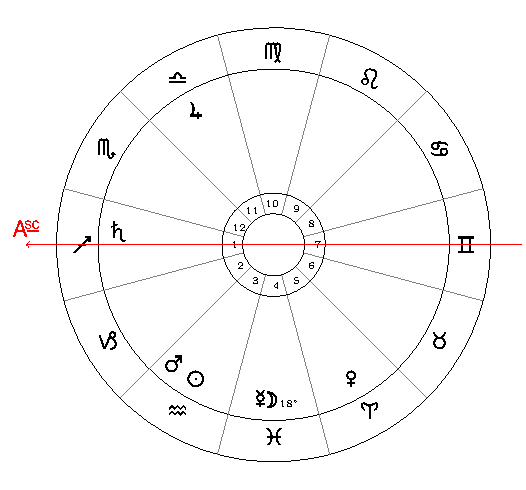
\includegraphics[width=.68\textwidth]{charts/6_6_1}
\caption{Chart 72 [VI.6.1, GH L132]}
\label{fig:chart72}
\end{wrapfigure}

The stars were arranged thus, in order in increasing longitude\footnote{Starts with the \Moon\, and then moves around the chart in sign order: \Moon, \Venus, \Jupiter, Ascendant, \Saturn, \Mars, \Sun, \Mercury}. We are investigating 52 years plus the time to Payni \textsl[...] 15 of the 53rd year <=52 years, 4 months, 3 days>. 

Now in this type of distribution the days and the cycles are calculated using 360-day periods, but the years of a nativity are calculated using 365 1/4 periods. Therefore I multiply the whole years, 52, by 5 1/4 for a total of 273. Then from Mechir 12 <the birth date> to Payni 15 there are 124 days. The grand total is 397 days. I subtract one circle <=one year> and the remaining days total 37. Since the birth was at night, the \Moon\, was considered the apheta of the overall chronocratorships. It was at IC, in a feminine sign in a triangle of a sect member <\Pisces\, - \Cancer\, - \Scorpio  the triangle of \Venus>, and appropriately situated. So the \Moon\, took 10 years 9 months of the given number of years first, then \Venus\, in \Aries\, 10 years 9 months, \textsl{[then \Jupiter\, in \Libra\, 10 years 9 months,]} then \Saturn\, in \Sagittarius 10 years 9 months. So far there have been 4 cycles, or 43 years.

Next follows \Mars. Its cycle of 10 years 9 months would make 53 years 9 months total, which is more than the given number of years under investigation. So I resorted to calculating by months, and gave to \Mars\, itself, as the ruler of the cycle, 15 months, adding this to the previous total for the fourth cycle, 43 years. Now the running total is 44 years 3 months. 

Next, <I give> to the \Sun\, 1 year 7 months, to \Mercury\, 20 months, to the \Moon\, 25 months, to \Venus\, 8 months, and to \Jupiter\, 12 months. So far, the total is is 51 years 3 months. 

Next \Saturn\, has 30 months to complete \Mars’s cycle, for a grand total of 53 years 9 months. But since this figure as well exceeds the given number of years, I count off the days as follows: including the period of \Jupiter\, the total was 51 years 3 months. I took the remaining days of the 52nd year (270) and of the 53rd year (360) and of the 54th year (37). 

The total is 667, with \Saturn\, receiving from \Mars. /\textbf{254K/} From this total \Saturn\, gives itself, in the first subsequent cycle, \textbf{/243P/} 129 days. Then it transfers the second cycle of a like 129 days to \Mars, and that star assigns itself its own days. The \Sun\, takes the third cycle next from \Saturn\, and assigns itself 129 days, then \Mercury\, the fourth, and the \Moon\, the fifth, both assigning themselves 129 days. Twenty-two days remain for the sixth cycle, which belongs to \Venus. \Venus\, assigns itself 8 days, then 12 days to \Jupiter. The remaining 2 days until the day in question belong to \Saturn. 

The overall chronocrator of the years was \Mars\, receiving from the \Moon. The chronocrator of the months was \Saturn\, receiving from \Mars. The chronocrator of the days was \Venus\, receiving the cycle from \Saturn. 

Consequently in the native’s 53rd year the grievous death of his wife occurred. Dangerous diseases and fines came on him. In the days under discussion, the native was condemned in a suit on behalf of his wife against a woman about legacies, about old matters, and he was oppressed by the great and was in nearly mortal danger. He had grief for his own family and for others’, so great as to turn to despair.
He was entangled in other precarious actions subject to penalties. For \Saturn\, still held the chronocratorship, not in its own sect, being in the Ascendant, and having the \Moon\, (the apheta) and \Mercury\, in inferior aspect <square to the left>. As a result many forgeries accompanied him, as well as lies, deceptions, many expenses, and dangerous diseases.


\newpage